%\documentclass[cprs.tex]{subfiles}
\setlength{\parskip}{1em}
\section*{Instructions for Part 3}

You are in a similar decision-making situation as in Part 1, but with the following exception:

\noindent In part 3, a forest fire occurred right at the beginning. This means that the forest size of 100 trees is reduced by 50\%, so that only 100 × 0.5 = 50 trees remain.

\noindent So your group does not start the game with 100 trees, but with 50 trees.

\noindent Your decision situation is as in part 1, with one exception:

\noindent The maximum number of trees that you can take in each round now depends on the number of trees at the beginning of the round. The maximum number of trees that you can find in a round is listed in the following table:

\noindent Current number of trees per round	 Maximum number of trees per group member

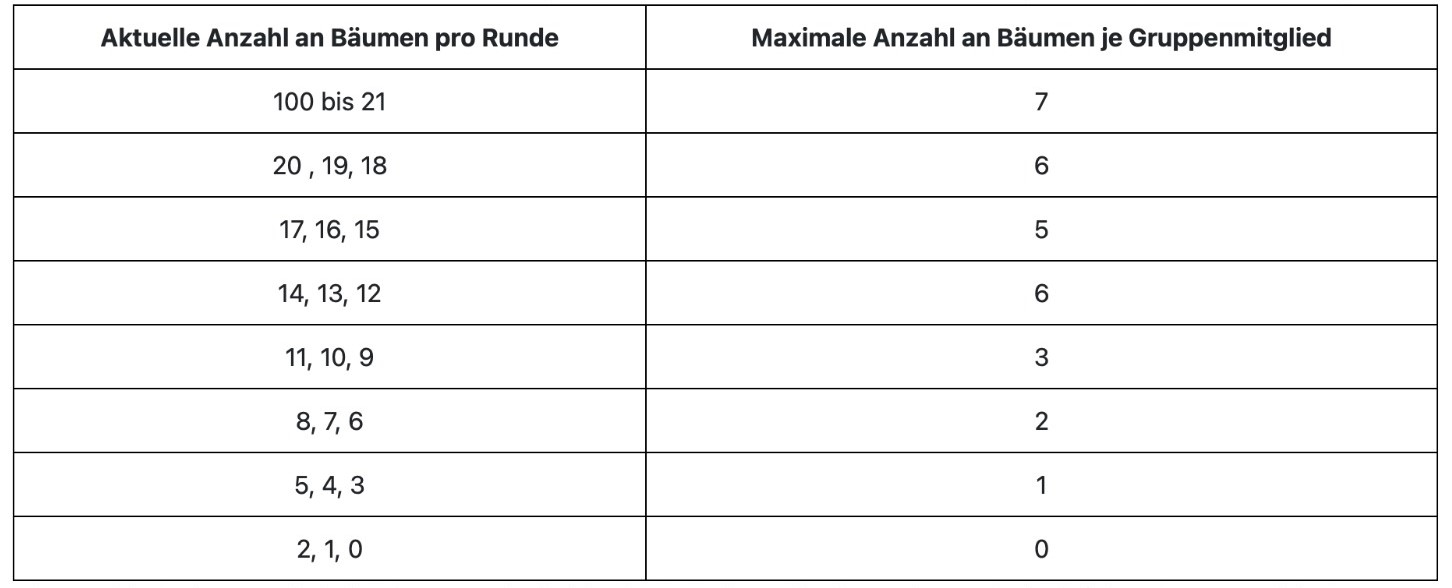
\includegraphics[width=16cm]{../bld/graphs/A. Harvest table.jpg}

\noindent The maximum number of trees that each group member may take in a round will be communicated to your group on the decision screen.

\noindent If the community forest falls below 3 trees in any round, you and your group members cannot remove the remaining trees, unless the forest grows back to at least 3 trees in the following rounds.

\noindent Otherwise, there are no changes compared to part 1. Your group will remain the same as before.
